\pgfplotsset{compat=1.17} % Use the version of pgfplots you have installed

\begin{figure}[htb]
    \centering
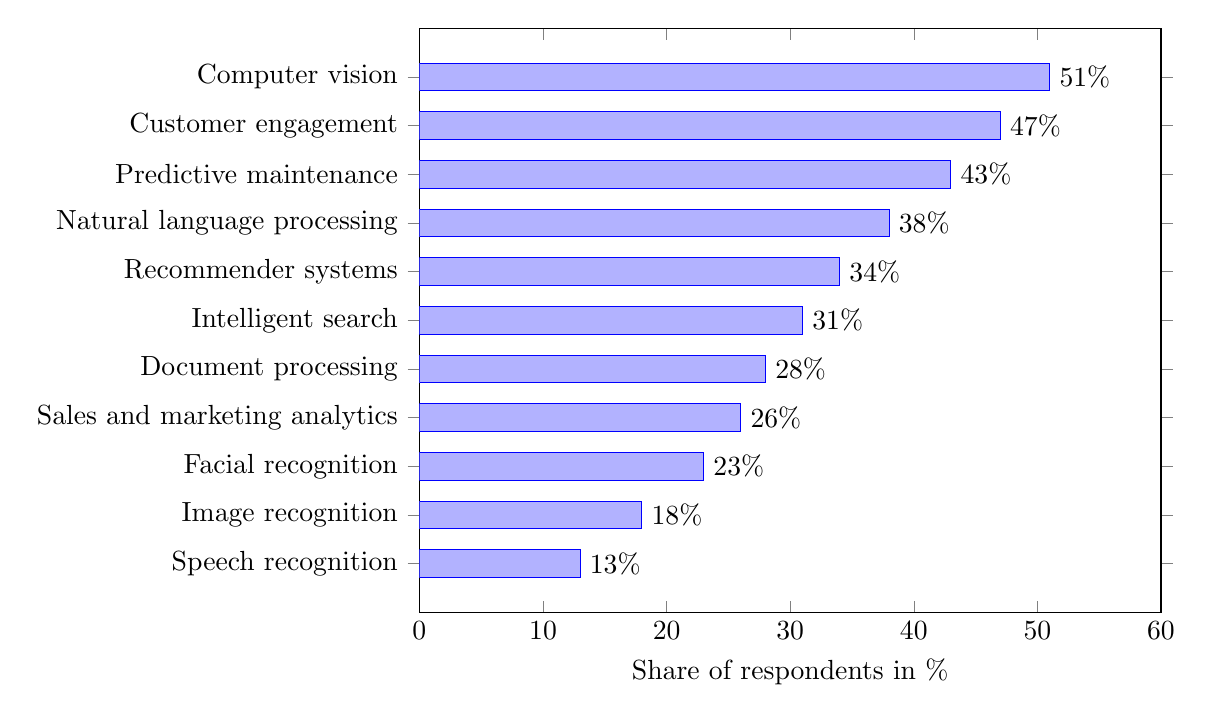
\begin{tikzpicture}
    \begin{axis}[
        xbar, % Horizontal bars
        xmin=0, xmax=60, % Set the minimum and maximum x-coordinates
        width=11cm, height=9cm, % Width and height of the plot
        enlarge y limits=0.1, % Add some space between bars
        xlabel={Share of respondents in \%}, % Label for the x-axis
        symbolic y coords={
            Speech recognition,
            Image recognition,
            Facial recognition,
            Sales and marketing analytics,
            Document processing,
            Intelligent search,
            Recommender systems,
            Natural language processing,
            Predictive maintenance,
            Customer engagement,
            Computer vision
        },
        ytick=data, % Use the data for y-ticks
        nodes near coords,
        nodes near coords align={anchor=west}, % Add the percentage labels near the bars% Align the labels horizontally
        point meta=explicit symbolic % The meta data is explicitly given as symbolic text
    ]
    \addplot [draw=blue,fill=blue!30 ] coordinates {
        (51,Computer vision)[51\%]
        (47,Customer engagement)[47\%]
        (43,Predictive maintenance)[43\%]
        (38,Natural language processing)[38\%]
        (34,Recommender systems)[34\%]
        (31,Intelligent search)[31\%]
        (28,Document processing)[28\%]
        (26,Sales and marketing analytics)[26\%]
        (23,Facial recognition)[23\%]
        (18,Image recognition)[18\%]
        (13,Speech recognition)[13\%]};
    \end{axis}
\end{tikzpicture}
\caption[Gängigste Verwendungszwecke von KI in Unternehmen]{Gängigsten Verwendungszwecke von KI in Unternehmen\footnotemark} % Caption for the figure
    \label{fig:ai_tech_distribution} % Label for referencing the figure
\end{figure}
\footnotetext{Entnommen aus: \cite{rackspace_most_2023}}